\documentclass[conference]{IEEEtran}
\IEEEoverridecommandlockouts


% Phil's macros
% Create code font alias
\usepackage{tikz}
% Code
\usepackage{listings}
\usepackage{xcolor}
\newcommand{\code}[1]{\texttt{#1}}
\usepackage{minted}
\usepackage{algorithm}
\usepackage{algorithmicx}
\usepackage[noend]{algpseudocode}
\usemintedstyle{trac}
\renewcommand\algorithmicdo{}
\renewcommand\algorithmicthen{}


\lstdefinestyle{customc}{
belowcaptionskip=1\baselineskip,
breaklines=true,
frame=L,
xleftmargin=\parindent,
language=C,
showstringspaces=false,
basicstyle=\footnotesize\ttfamily,
keywordstyle=\bfseries\color{green!40!black},
commentstyle=\itshape\color{purple!40!black},
identifierstyle=\color{blue},
stringstyle=\color{orange},
columns=fullflexible,
language=c,
frame=true,
numbers=left
}
\lstdefinestyle{snippet}{
belowcaptionskip=1\baselineskip,
breaklines=true,
frame=L,
xleftmargin=\parindent,
language=C,
showstringspaces=false,
basicstyle=\footnotesize\ttfamily,
keywordstyle=\bfseries\color{green!40!black},
commentstyle=\itshape\color{purple!40!black},
identifierstyle=\color{blue},
stringstyle=\color{orange},
columns=fullflexible,
language=c
}
\lstdefinestyle{hex}{
belowcaptionskip=1\baselineskip,
breaklines=true,
frame=LR,
% xleftmargin=\parindent,
language=C,
showstringspaces=false,
basicstyle=\footnotesize\ttfamily,
keywordstyle=\bfseries\color{green!40!black},
commentstyle=\itshape\color{purple!40!black},
% identifierstyle=\color{blue},
stringstyle=\color{orange},
columns=fullflexible,
keywords=[2]{fail},
keywords=[3]{pass},
keywordstyle={\color{blue!80!black}},
keywordstyle=[2]{\color{red!80!black}},
keywordstyle=[3]{\color{green!50!black}},
}

\lstdefinestyle{asm}{
belowcaptionskip=1\baselineskip,
breaklines=true,
frame=L,
xleftmargin=\parindent,
language=[x86masm]Assembler,
showstringspaces=false,
basicstyle=\footnotesize\ttfamily,
keywordstyle=\bfseries\color{green!40!black},
commentstyle=\itshape\color{purple!40!black},
identifierstyle=\color{blue},
stringstyle=\color{orange},
columns=fullflexible,
}


% The preceding line is only needed to identify funding in the first footnote. If that is unneeded, please comment it out.
\usepackage{cite}
\usepackage{amsmath,amssymb,amsfonts}
\usepackage{algorithmic}
\usepackage{graphicx}
\usepackage{textcomp}
\def\BibTeX{{\rm B\kern-.05em{\sc i\kern-.025em b}\kern-.08em
T\kern-.1667em\lower.7ex\hbox{E}\kern-.125emX}}
\begin{document}

\title{Breaking Trivium with Stuck-at-0 Faults}

\author{\IEEEauthorblockN{Phillip Gajland}
\IEEEauthorblockA{\textit{KTH Royal Institute of Technology} \\
\textit{Theoretical Computer Science} \\
Stockholm, Sweden \\
gajland@kth.se}
\and
\IEEEauthorblockN{Daniel Skantz}
\IEEEauthorblockA{\textit{KTH Royal Institute of Technology} \\
\textit{Theoretical Computer Science} \\
Stockholm, Sweden \\
danska@kth.se}
\and
\IEEEauthorblockN{Elena Dubrova}
\IEEEauthorblockA{\textit{KTH Royal Institute of Technology} \\
\textit{Electronic Systems Design} \\
Stockholm, Sweden \\
dubrova@kth.se}
}

\maketitle

\begin{abstract}
As the Internet of Things (IoT) continues to gain traction, so does the need for secure IoT devices. Although 23.3 billion IoT devices are estimated to be connected by 2023 \cite{iot}, vendors often neglect the security of such devices. Stream ciphers can offer an attractive solution for secure communications, when low power consumption is essential. 

The eSTREAM project was intended to \textit{"identify new stream ciphers suitable for widespread adoption"}.\cite{call} In 2018, Trivium, a synchronous stream cipher was selected as part of the portfolio for low area hardware ciphers. 

In this paper we study the design choices made by the authors of Trivium in order to demonstrate a fault attack on the software implementation of the cipher. Whilst Trivium maintains most desirable cryptographic properties, a simple design was chosen by the authors to provide flexibility. Our attack works by modifying the compiled binary at targeted positions to introduce stuck at 0 faults. Using this technique, we are able to reduce the non-linear feedback function to a linear one. Thus, it is possible to recover the 288-bit internal state of the cipher. In turn extraction of the 80-bit key becomes tractable.
\end{abstract}

\begin{IEEEkeywords}
trivium, stream cipher, fault attack
\end{IEEEkeywords}

\section{Introduction}




In this paper we analyse the design choices made by the authors of Trivium, in order to discover a new class of vulnerabilities. 


We go on to demonstrate a fault attack on the software implementation of Trivium.

As the Internet of Things (IoT) continues to gain traction, so does the need for secure IoT devices. Although 23.3 billion IoT devices are estimated to be connected by 2023 \cite{iot}, vendors often neglect the security of such devices. Stream ciphers can offer an attractive solution for secure communications, when low power consumption is essential. 

The eSTREAM project was intended to \textit{"identify new stream ciphers suitable for widespread adoption"}.\cite{call} In 2018, Trivium, a synchronous stream cipher was selected as part of the portfolio for low area hardware ciphers. In this paper we analyse the design choices made by the authors of Trivium. We go on to demonstrate a fault attack on the software implementation of Trivium. 

The attack works by modifying compiled binaries at targeted positions to introduce stuck at 0 faults. Using this technique, we are able to reduce the non-linear feedback function to a linear one. Thus, it is possible to recover the 288-bit internal state of the cipher and in turn extraction of the 80-bit key becomes tractable.


trade off between performance and security, when low power consumption is of high significance. 


Stream ciphers can offer an attractive trade off between security and per in situations where power consutmption 
, due to their low


When performance 

A primary concern is securing systems 

an attractive solution when low powerconsumption is vital 
Thus, significantly increasing the attack surface for adversaries to mount attacks on larger systems, as was demonstrated in the 2016 Dyn cyberattack.


Stream Ciphers offer an attractive trade-off between lightweight crypto primitives and security in 

\section{Background}

As a result of the failures of all six stream ciphers submitted to the NESSIE (New European Schemes for Signatures, Integrity and Encryption) project, in 2004 the eSTREAM project was launched in order to \textit{"identify new stream ciphers suitable for widespread adoption"}\cite{call}.



\section{Ease of Use}

\subsection{Code Analysis}
The official C code authored by Christophe De Canni\`ere can be found on  

In the C code the \code{UPDATE()} macro originally does the following
\begin{lstlisting}[style=snippet]
#define UPDATE()
do { 
T(1) = S64(1, 66) ^ S64(1, 93);
T(2) = S64(2, 69) ^ S64(2, 84);
T(3) = S64(3, 66) ^ S96(3, 111);

Z(T(1) ^ T(2) ^ T(3));

T(1) ^= (S64(1, 91) & S64(1, 92)) ^ S64(2, 78); 
T(2) ^= (S64(2, 82) & S64(2, 83)) ^ S64(3, 87); 
T(3) ^= (S96(3, 109) & S96(3, 110)) ^ S64(1, 69); 
} while (0)
\end{lstlisting}
However, our fault injection is done as follows in the C code.
\begin{lstlisting}[style=snippet]
#define UPDATE()
do {
.       .       .
.       .       .
.       .       .
T(1) ^= S64(1, 91) ^ S64(2, 78); 
T(2) ^= S64(2, 82) ^ S64(3, 87); 
T(3) ^= S96(3, 109) ^ S64(1, 69); 
} while (0)
\end{lstlisting}

The \code{UPDATE()} macro is used in the \code{ECRYPT\_ivsetup} and \code{ECRYPT\_process\_bytes} functions. This means that when disassembling the \code{trivium.o} object file 

We run the fault injected code using the following key \code{0x0F62B5085BAE0154A7FA} and IV \code{0x288FF65DC42B92F960C7}. Using the Berlekamp–Massey algorithm \cite{massey} we find the shortest linear feedback register (LFSR) for the given bitstream. The polynomial is
$x^{61} + x^{60} + x^{55} + x^{54} + x^{52} + x^{51} + x^{46} + x^{45} + x^{43} + x^{42} + x^{41} + x^{40} + x^{39} + x^{38} + x^{37} + x^{36} + x^{35} + x^{31} + x^{28} + x^{25} + x^{24} + x^{23} + x^{20} + x^{19} + x^{18} + x^{11} + x^8 + x^7 + 1$.

original
\begin{lstlisting}[style=hex]
........ EA0421F2 894DBC89 ........ 0FA4F80D
31D121F0 448B65C8 ........ 6DCC440F A4EB1B21
C74431D3 31FB895D ........ 89D30FA4 F30421C3
448B5DC8 ........ E0440FA4 F00921DF 89C34431
........ 13450FA4 E7124121 C74489C0 4131CF45
........ F24589E7  F10E4121 F9448975 C8440FA4
........ 410FA4D7 124121C7 ........  ........
\end{lstlisting}

modified
\begin{lstlisting}[style=hex]
........ EA0433F6 894DBC89 ........ 0FA4F80D 
31D133F6 448B65C8 ........ 6DCC440F A4EB1B33
C04431D3 31FB895D ........ 89D30FA4 F30433C0 
448B5DC8 ........ E0440FA4 F00933C9 89C34431
........ 13450FA4 E71233C0 904489C0 4131CF45
........ F24589E7 F10E33FF 90448975 C8440FA4 
........ 410FA4D7 1233C090 ........  ........
\end{lstlisting}



original
modified
\newcommand{\hf}{\makebox[0pt][l]{\color{green}\rule[-3pt]{0.08\linewidth}{11pt}}}
\newcommand{\ha}{\makebox[0pt][l]{\color{green}\rule[-3pt]{0.04\linewidth}{11pt}}}

\begin{lstlisting}[style=hex,escapechar=\%]
1a) ORIG:...    EA0421F2 ........ 31D121F0 ........
1b) MOD:....     EA04%\hf%33F6 ........ 31D1%\hf%33F6  ........

2a)  A4EB1B21 C74431D3 ........ F30421C3
2b)  A4EB1B%\ha%33 %\ha%C04431D3 ........ F304%\hf%33C0

3a) ........ F00921DF ........ E7124121 C74489C0
3b) ........ F009%\hf%33C9 ........ E712%\hf%33C0 %\ha%904489C0 

4a) ........ F10E4121 F9448975 ........ F00D21C8

124121C7
4b) ........ F10E%\hf%33FF %\ha%90448975 ........ F00D33C9

12%\hf%33C0%\ha%90
\end{lstlisting}

\clearpage

\begin{lstlisting}[style=asm]
and    %esi,%edx    ---> 21 f2 
and    %esi,%eax    ---> 21 f0
and    %eax,%edi    ---> 21 c7 

and    %eax,%ebx    ---> 21 c3
and    %ebx,%edi    ---> 21 df 
and    %eax,%r15d   --> 41 21 c7

and    %edi,%r9d    ---> 41 21 f9
and    %ecx,%eax    ---> 21 c8
and    %eax,%r15d   --> 41 21 c7
\end{lstlisting}

\begin{lstlisting}[style=asm]
xor    %esi,%esi    ---> 33 f6
xor    %esi,%esi    ---> 33 f6
xor    %eax,%eax    ---> 33 c0

xor    %eax,%eax    ---> 33 c0
xor    %ebx,%ebx    ---> 33 db 
xor    %eax,%eax    ---> 33 c0
nop     ------------->  90

xor    %edi,%edi    ---> 33 ff
nop     -------------> 90
xor    %ecx,%ecx    ---> 33 c9
xor    %eax,%eax    ---> 33 c0
nop     -------------> 90
\end{lstlisting}


A linear system with $k$ variables can be solved in time $k^\omega$, where $\omega \leq 2.376$.
So in our case finding the solution takes at most $288^{2.376} \leq 697,456$ operations


\subsection{Unwinding the bitstream}







\subsection{presentation}


\begin{itemize}
\item[$\blacktriangleright$] A network is only as secure as its weakest link.
\item[$\blacktriangleright$] 23.3 billion IoT devices by 2023.
\item[$\blacktriangleright$] Need for securing IoT devices.
\begin{itemize}[itemsep=0.25cm]
\item[$\triangleright$] DDoS attacks e.g. Dyn cyberattack 2016.
\end{itemize}
\item[$\blacktriangleright$] Require energy efficient ciphers.
\end{itemize}

\begin{itemize}
\item[$\blacktriangleright$] \textbf{eSTREAM project} - 2004
\begin{itemize}
\item Organised by ECRYPT to \textit{"identify new stream ciphers suitable for widespread adoption"}.
\end{itemize}
\item[$\blacktriangleright$] \textbf{eSTREAM portfolio} - 2008/2011
\begin{table}
\centering
\begin{tabular}{l|l}
Profile 1 (software) & Profile 2 (hardware)\\\hline
HC-128 & Grain\\
Rabiit & MICKEY\\
Salsa20 & Trivium\\
SOSEMANUK &
\end{tabular}
\end{table}
\end{itemize}

\begin{itemize}
\item[$\blacktriangleright$] Key: 80-bit key
\item[$\blacktriangleright$] Initialisation Vector: 80-bit
\item[$\blacktriangleright$] Output: $\leq2^{64}-bit$
\item[$\blacktriangleright$] Internal State: 288-bit
\item[$\blacktriangleright$] 3 shift registers:
\begin{itemize}
\item a) 93-bit
\item b) 84-bit
\item c) 111-bit
\end{itemize}
\end{itemize}
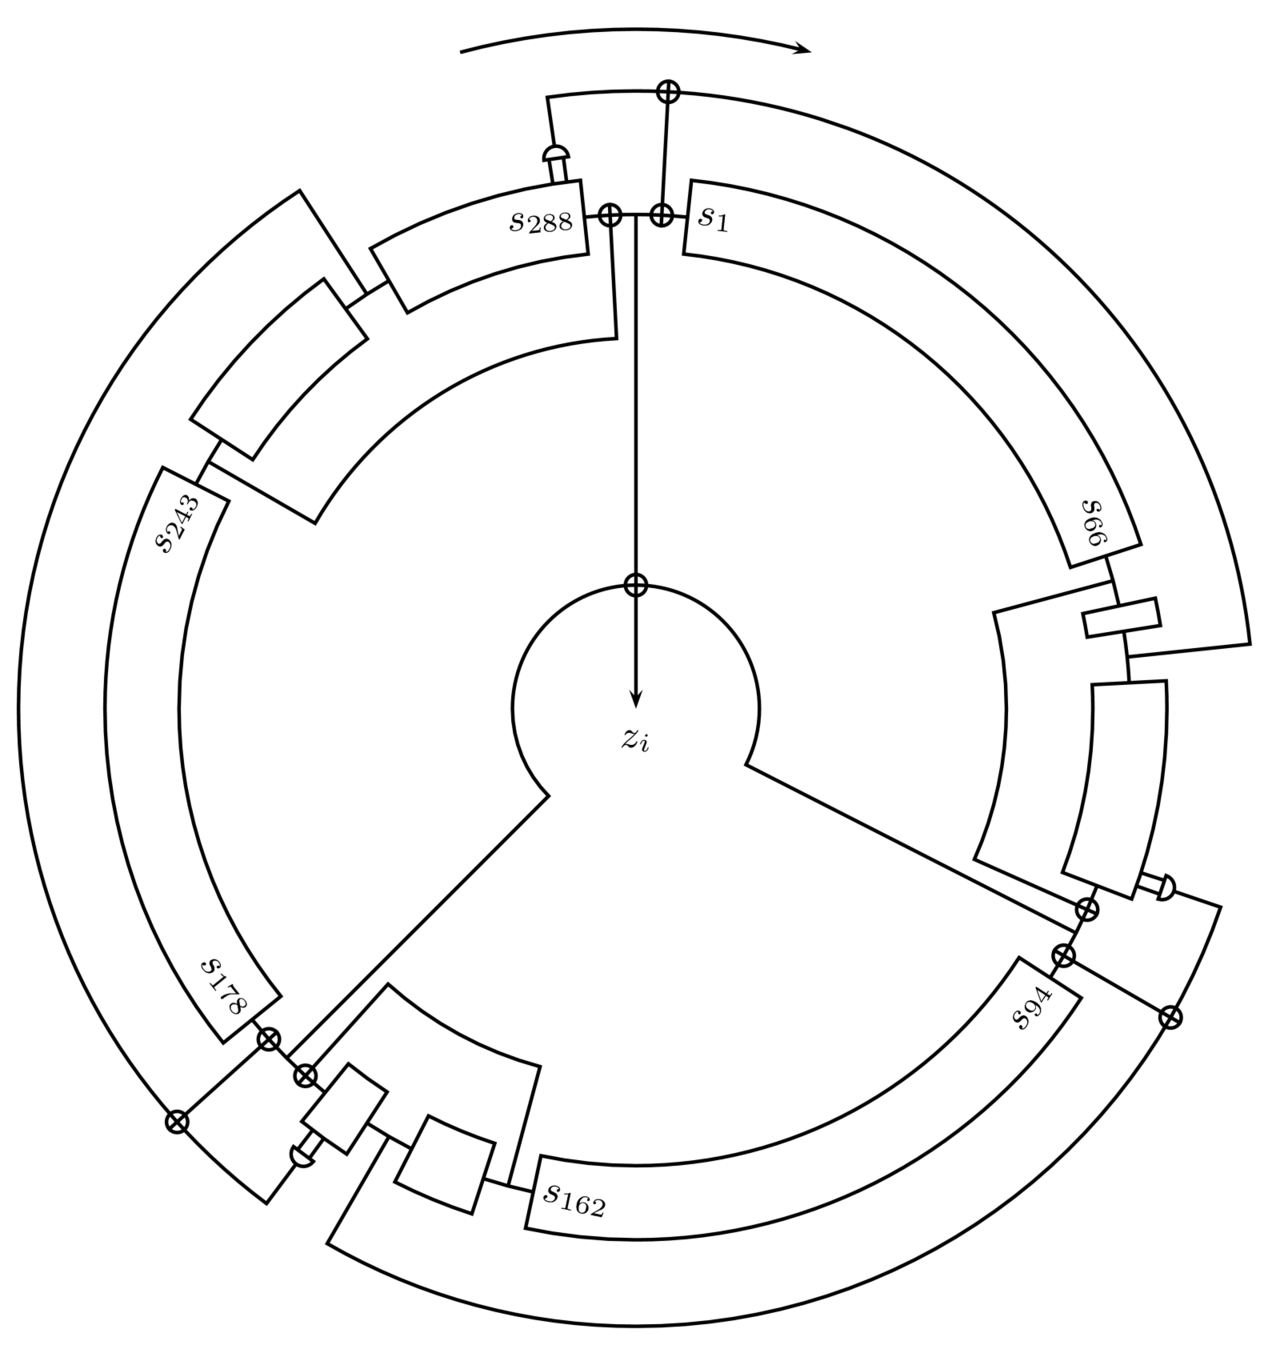
\includegraphics[width=0.4\textwidth]{figures/round.png}\cite{circle}


\begin{algorithm}[H]
\begin{algorithmic}[1]
\For{$i=1$ to $N$} \Comment{$N\leq 2^{64}$}
\State $t_1 \gets s_{66} + s_{93}$
\State $t_2 \gets s_{162} + s_{177}$
\State $t_3 \gets s_{243} + s_{288}$
\State
\State $z_i \gets t_1 + t_2 + t_3$
\State
\State $t_1 \gets t_1 + s_{91} \cdot s_{92} + s_{171}$
\State $t_2 \gets t_2 + s_{175} \cdot s_{176} + s_{264}$
\State $t_3 \gets t_3 + s_{286} \cdot s_{287} + s_{69}$
\State
\State $(s_1,s_2,\dots,s_{93}) \gets (t_3,s_1,\dots,s_{92})$
\State $(s_{94},s_{95},\dots,s_{177}) \gets (t_1,s_{94},\dots,s_{176})$
\State $(s_{178},s_{179},\dots,s_{288}) \gets (t_2,s_{178},\dots,s_{287})$
\EndFor
\end{algorithmic}
\end{algorithm}

Key and IV setup
\begin{itemize}
\item[$\blacktriangleright$] Run over 4 full cycles
\end{itemize}
\begin{algorithm}[H]
\begin{algorithmic}[1]
\State $(s_1,s_2,\dots,s_{93}) \gets (K_1,\dots,K_{80},0,\dots,0)$
\State $(s_{94},s_{95},\dots,s_{177}) \gets (IV_1,\dots,IV_{80},0,\dots,0)$
\State $(s_{178},s_{179},\dots,s_{288}) \gets (0,\dots,0,1,1,1)$
\State
\For{$i=1$ to $4\cdot288$}
\State $t_1 \gets s_{66} + s_{91} \cdot s_{92} + s_{93} + s_{171}$
\State $t_2 \gets s_{162} + s_{175} \cdot s_{176} + s_{177} + s_{264}$
\State $t_3 \gets s_{243} + s_{286} \cdot s_{287} + s_{288}+ s_{69}$
\State
\State $(s_1,s_2,\dots,s_{93}) \gets (t_3,s_1,\dots,s_{92})$
\State $(s_{94},s_{95},\dots,s_{177}) \gets (t_1,s_{94},\dots,s_{176})$
\State $(s_{178},s_{179},\dots,s_{288}) \gets (t_2,s_{178},\dots,s_{287})$
\EndFor
\end{algorithmic}
\end{algorithm}


\section{Attack Scenario}

Stuck-at-0 Faults
\begin{itemize}
\item[$\blacktriangleright$] Injecting stuck-at-0 faults can be done in multiple ways.
\begin{itemize}
\item[$\triangleright$] Binary code modification,
\item[$\triangleright$] FPGA bitsream modification,
\item[$\triangleright$] EM fault injection, 
\item[$\triangleright$] Optical fault injection. 
\end{itemize}
\end{itemize}


Assumptions
\begin{itemize}
\item[$\blacktriangleright$] Physical access to device; e.g. during shipment.
\item[$\blacktriangleright$] Proprietary protection mechanism, preventing arbitrary code from being run.
\item[$\blacktriangleright$] Code being executed on device is not signed.
\item[$\blacktriangleright$] Lock bits need to protect against read-back are not set.
\item[$\blacktriangleright$] Key is securely stored and cannot be obtained with ease.
\item[$\blacktriangleright$] Key is reused.
\end{itemize}


Procedure
\begin{itemize}
\item[$\blacktriangleright$] Load fault injected binary onto device.
\item[$\blacktriangleright$] Run fault injected Trivium to obtain $\alpha$ output bits.
\item[$\blacktriangleright$] Cryptanalyse output stream and recover key.
\item[$\blacktriangleright$] Load original binary onto device.
\item[$\blacktriangleright$] Future communications can be deciphered as the key is known.
\end{itemize}

\section{Fault Injection}

Fault Injection
\begin{figure}
\includestandalone[width=0.45\textwidth]{figures/modified}
\end{figure}











Number equations consecutively. To make your
equations more compact, you may use the solidus (~/~), the exp function, or
appropriate exponents. Italicize Roman symbols for quantities and variables,
but not Greek symbols. Use a long dash rather than a hyphen for a minus
sign. Punctuate equations with commas or periods when they are part of a
sentence, as in:
\begin{equation}
a+b=\gamma\label{eq}
\end{equation}

Be sure that the
symbols in your equation have been defined before or immediately following
the equation. Use ``\eqref{eq}'', not ``Eq.~\eqref{eq}'' or ``equation \eqref{eq}'', except at
the beginning of a sentence: ``Equation \eqref{eq} is . . .''

\subsection{\LaTeX-Specific Advice}

Please use ``soft'' (e.g., \verb|\eqref{Eq}|) cross references instead
of ``hard'' references (e.g., \verb|(1)|). That will make it possible
to combine sections, add equations, or change the order of figures or
citations without having to go through the file line by line.

Please don't use the \verb|{eqnarray}| equation environment. Use
\verb|{align}| or \verb|{IEEEeqnarray}| instead. The \verb|{eqnarray}|
environment leaves unsightly spaces around relation symbols.

Please note that the \verb|{subequations}| environment in {\LaTeX}
will increment the main equation counter even when there are no
equation numbers displayed. If you forget that, you might write an
article in which the equation numbers skip from (17) to (20), causing
the copy editors to wonder if you've discovered a new method of
counting.

{\BibTeX} does not work by magic. It doesn't get the bibliographic
data from thin air but from .bib files. If you use {\BibTeX} to produce a
bibliography you must send the .bib files.

{\LaTeX} can't read your mind. If you assign the same label to a
subsubsection and a table, you might find that Table I has been cross
referenced as Table IV-B3.

{\LaTeX} does not have precognitive abilities. If you put a
\verb|\label| command before the command that updates the counter it's
supposed to be using, the label will pick up the last counter to be
cross referenced instead. In particular, a \verb|\label| command
should not go before the caption of a figure or a table.

Do not use \verb|\nonumber| inside the \verb|{array}| environment. It
will not stop equation numbers inside \verb|{array}| (there won't be
any anyway) and it might stop a wanted equation number in the
surrounding equation.

\subsection{Some Common Mistakes}\label{SCM}
\begin{itemize}
\item The word ``data'' is plural, not singular.
\item The subscript for the permeability of vacuum $\mu_{0}$, and other common scientific constants, is zero with subscript formatting, not a lowercase letter ``o''.
\item In American English, commas, semicolons, periods, question and exclamation marks are located within quotation marks only when a complete thought or name is cited, such as a title or full quotation. When quotation marks are used, instead of a bold or italic typeface, to highlight a word or phrase, punctuation should appear outside of the quotation marks. A parenthetical phrase or statement at the end of a sentence is punctuated outside of the closing parenthesis (like this). (A parenthetical sentence is punctuated within the parentheses.)
\item A graph within a graph is an ``inset'', not an ``insert''. The word alternatively is preferred to the word ``alternately'' (unless you really mean something that alternates).
\item Do not use the word ``essentially'' to mean ``approximately'' or ``effectively''.
\item In your paper title, if the words ``that uses'' can accurately replace the word ``using'', capitalize the ``u''; if not, keep using lower-cased.
\item Be aware of the different meanings of the homophones ``affect'' and ``effect'', ``complement'' and ``compliment'', ``discreet'' and ``discrete'', ``principal'' and ``principle''.
\item Do not confuse ``imply'' and ``infer''.
\item The prefix ``non'' is not a word; it should be joined to the word it modifies, usually without a hyphen.
\item There is no period after the ``et'' in the Latin abbreviation ``et al.''.
\item The abbreviation ``i.e.'' means ``that is'', and the abbreviation ``e.g.'' means ``for example''.
\end{itemize}
An excellent style manual for science writers is \cite{b7}.

\subsection{Authors and Affiliations}
\textbf{The class file is designed for, but not limited to, six authors.} A
minimum of one author is required for all conference articles. Author names
should be listed starting from left to right and then moving down to the
next line. This is the author sequence that will be used in future citations
and by indexing services. Names should not be listed in columns nor group by
affiliation. Please keep your affiliations as succinct as possible (for
example, do not differentiate among departments of the same organization).

\subsection{Related Works}
Dubrova performed some ground breaking work by demonstrating a single fault attack on ACORN.



\subsection{Figures and Tables}
\paragraph{Positioning Figures and Tables} Place figures and tables at the top and
bottom of columns. Avoid placing them in the middle of columns. Large
figures and tables may span across both columns. Figure captions should be
below the figures; table heads should appear above the tables. Insert
figures and tables after they are cited in the text. Use the abbreviation
``Fig.~\ref{fig}'', even at the beginning of a sentence.

\begin{table}[htbp]
\caption{Table Type Styles}
\begin{center}
\begin{tabular}{|c|c|c|c|}
\hline
\textbf{Table}&\multicolumn{3}{|c|}{\textbf{Table Column Head}} \\
\cline{2-4}
\textbf{Head} & \textbf{\textit{Table column subhead}}& \textbf{\textit{Subhead}}& \textbf{\textit{Subhead}} \\
\hline
copy& More table copy$^{\mathrm{a}}$& &  \\
\hline
\multicolumn{4}{l}{$^{\mathrm{a}}$Sample of a Table footnote.}
\end{tabular}
\label{tab1}
\end{center}
\end{table}



\begin{figure}[htb]
\centering
\resizebox{0.5\textwidth}{!}{\tikzset{XOR/.style={draw,circle,append after command={
[shorten >=\pgflinewidth, shorten <=\pgflinewidth,]
(\tikzlastnode.north) edge (\tikzlastnode.south)
(\tikzlastnode.east) edge (\tikzlastnode.west)
}
}
}

\tikzset{wire/.style = {thick,rounded corners=1.5pt}}
\tikzset{AND/.style={draw, circle}}
\tikzset{DOT/.style={ fill, circle, inner sep=0cm, minimum size=1.5mm}}



\begin{tikzpicture}[
roundnode/.style={circle, draw=green!60, fill=green!5, very thick, minimum size=7mm},
square/.style={rectangle, minimum size=1cm},
]

    \node[square,draw] (1) at (2,11) {$s_1$};
    \draw (2.5,10.5) rectangle (4.5,11.5);
    \node[square,draw] (66) at (5,11) {$s_{66}$};
    \node[square,draw] (empty) at (6,11) {};
    \node[square,draw] (69) at (7,11) {$s_{69}$};
    \node[square,draw] (empty) at (8,11) {};
    \node[square,draw] (91) at (9,11) {$s_{91}$};
    \node[square,draw] (92) at (10,11) {$s_{92}$};
    \node[square,draw] (93) at (11,11) {$s_{93}$};

    \node[square,draw] (94) at (2,7) {$s_{94}$};
    \draw (2.5,6.5) rectangle (4.5,7.5);
    \node[square,draw] (162) at (5,7) {$s_{162}$};
    \node[square,draw] (empty) at (6,7) {};
    \node[square,draw] (171) at (7,7) {$s_{171}$};
    \node[square,draw] (empty) at (8,7) {};
    \node[square,draw] (175) at (9,7) {$s_{175}$};
    \node[square,draw] (176) at (10,7) {$s_{176}$};
    \node[square,draw] (177) at (11,7) {$s_{177}$};
    \node[XOR] (x177) at (11,8) {};

    \node[square,draw] (178) at (2,3) {$s_{178}$};
    \draw (2.5,2.5) rectangle (4.5,3.5);
    \node[square,draw] (243) at (5,3) {$s_{243}$};
    \node[square,draw] (empty) at (6,3) {};
    \node[square,draw] (264) at (7,3) {$s_{264}$};
    \node[square,draw] (empty) at (8,3) {};
    \node[square,draw] (286) at (9,3) {$s_{286}$};
    \node[square,draw] (287) at (10,3) {$s_{287}$};
    \node[square,draw] (288) at (11,3) {$s_{288}$};

    \node[XOR] (x93) at (11,12) {};
    \node[XOR] (x1) at (0,10) {};
    \node[XOR] (x171) at (7,9) {};
    \node[XOR] (z) at (13,8) {};
    \node[XOR] (x264) at (7,5) {};
    \node[XOR] (x288) at (11,4) {};
    \node[DOT] (d1) at (12,12) {};
    \node[DOT] (d2) at (12,8) {};
    \node[DOT] (d3) at (12,4) {};
    \node (zi) at (14,8) {$z_i$};
    \node (t1) at (13.3,10) {$t_1$};
    \node (t2) at (12.3,8.2) {$t_2$};
    \node (t3) at (13.3,6) {$t_3$};


    \draw[wire,->](x1)--(0,11)--(1);
    \draw[wire,->](66)--(5,12)--(x93);
    \draw[wire,->](69)--(7,10)--(x1);
    \draw[wire,->](93)--(x93);
    \draw[wire,->](x93)--(13,12)--(z);
    \draw[wire,->](d1)--(12,9)--(x171);

    \draw[wire,->](162)--(5,8)--(x177);
    \draw[wire,->](171)--(x171);
    \draw[wire,->](x171)--(1,9)--(1,7)--(94);
    \draw[wire,->](177)--(x177);
    \draw[wire,->](x177)--(z);
    \draw[wire,->](d2)--(12,5)--(x264);

    \draw[wire,->](243)--(5,4)--(x288);
    \draw[wire,->](264)--(x264);
    \draw[wire,->](x264)--(1,5)--(1,3)--(178);
    \draw[wire,->](288)--(x288);
    \draw[wire,->](x288)--(13,4)--(z);
    \draw[wire,->](d3)--(12,1)--(0,1)--(x1);

    \draw[wire,->](z)--(13.8,8);
\end{tikzpicture}
}
\caption{Modified Trivium Circuit}\label{fig:myfigure}
\end{figure}

Figure Labels: Use 8 point Times New Roman for Figure labels. Use words
rather than symbols or abbreviations when writing Figure axis labels to
avoid confusing the reader. As an example, write the quantity
``Magnetization'', or ``Magnetization, M'', not just ``M''. If including
units in the label, present them within parentheses. Do not label axes only
with units. In the example, write ``Magnetization (A/m)'' or ``Magnetization
\{A[m(1)]\}'', not just ``A/m''. Do not label axes with a ratio of
quantities and units. For example, write ``Temperature (K)'', not
``Temperature/K''.

\section*{Acknowledgment}

The preferred spelling of the word ``acknowledgment'' in America is without
an ``e'' after the ``g''. Avoid the stilted expression ``one of us (R. B.
G.) thanks $\ldots$''. Instead, try ``R. B. G. thanks$\ldots$''. Put sponsor
acknowledgments in the unnumbered footnote on the first page.

\begin{thebibliography}{00}
\bibitem{massey} Massey, J. L. (1969). Shift-Register Synthesis and BCH Decoding. IEEE Transactions on Information Theory, 15(1), 122–127. https://doi.org/10.1109/TIT.1969.1054260
\bibitem{call} "ECRYPT Call for Stream Cipher Primitives" (version 1.3 ed.). 12 April 2005. Retrieved 2 April 2014. http://www.ecrypt.eu.org/stream/call/
\bibitem{block-insp} Christophe De Cannière, Bart Preneel (2006-01-02). "Trivium - A Stream Cipher Construction Inspired by Block Cipher Design Principles"
\bibitem{iot} Ericsson, “Ericsson
Mobility Report” 2018. https://www.ericsson.com/49d1d9/assets/local/mobility-report/documents/2018/ericsson-mobility-report-june-2018.pdf
\end{thebibliography}

\end{document}
